\chapter{علم بهینه‌سازی کلاسیک}
در این فصل ابتدا به توضیح کلی مفاهیم بهینه‌سازی کلاسیک و کاربرد‌هایی از آن میپردازیم. سپس تاریخچه آن را از ابتدا تا کنون به صورت اجمالی بررسی مینماییم. در بخش بعد، به بررسی انواع توابع بهینه‌سازی و مسائل معروف آن میپردازیم. در نهایت نیز بهینه‌سازی کلاسیک و مدرن و کاربرد آنها در مخابرات را مورد بررسی قرار میدهیم.
\newpage
%%%%%%%%%%%%%%%%%%%%%%%%%%%%%%%%%%%%%%%%%%%
\section{
مقدمه‌ای بر بهینه سازی کلاسیک
}

\subsection{مفهوم بهینه‌سازی کلاسیک}

بهینه‌سازی کلاسیک یک حوزه ریاضی است که به مطالعه فرآیند یافتن مقدار کمینه یا بیشینه یک تابع هدف تحت قیدها می‌پردازد. این تابع هدف می‌تواند معمولاً معیاری از کیفیت یا کمیت یک سیستم یا فرآیند باشد که می‌خواهیم آن را بهینه کنیم. محدودیت‌ها معمولاً شرایط و قیودی هستند که می‌توانند بر روی متغیرهای مستقل تابع هدف اعمال شوند.

\subsection{کاربردهای بهینه‌سازی کلاسیک}

بهینه‌سازی کلاسیک در بخش‌های مختلف زمینه‌های علمی و مهندسی به کار می‌رود:

- \textbf{مهندسی صنایع و مدیریت:} در مسائل مدیریت موجودی، برنامه‌ریزی تولید و برنامه‌ریزی منابع، بهینه‌سازی کلاسیک به ما کمک می‌کند تا بهترین تصمیم‌ها را برای تخصیص منابع و اجرای عملیات انجام دهیم.

- \textbf{علوم کامپیوتر و مهندسی نرم‌افزار:} در طراحی الگوریتم‌ها و بهینه‌سازی عملکرد نرم‌افزارها، بهینه‌سازی کلاسیک به ما کمک می‌کند تا کارایی سیستم‌های نرم‌افزاری را افزایش دهیم.

- \textbf{مهندسی برق و مخابرات:} در طراحی شبکه‌ها، انتخاب پارامترهای سیستم‌های ارتباطی، و بهبود کیفیت انتقال اطلاعات، بهینه‌سازی کلاسیک به ما کمک می‌کند تا از منابع محدود بهره‌برداری بهتری داشته باشیم.

- \textbf{علوم زیستی:} در تحلیل داده‌های پزشکی و زیست‌شناسی، بهینه‌سازی کلاسیک می‌تواند در شناخت رفتار سیستم‌ها و تخمین پارامترهای مهم مورد استفاده قرار گیرد.

- \textbf{مهندسی مکانیک:} در طراحی سازه‌ها، بهینه‌سازی کلاسیک به ما کمک می‌کند تا بهترین ترازبندی و مواد مصرفی را برای ساخت و سازها انتخاب کنیم.

\subsection{روش‌های بهینه‌سازی}

برای حل مسائل بهینه‌سازی کلاسیک، از روش‌های مختلفی مانند روش‌های گرادیانی، روش‌های تکاملی، و روش‌های تقریبی استفاده می‌شود. این روش‌ها بسته به خصوصیات مسئله و محدودیت‌ها ممکن است ویژگی‌های متفاوتی داشته باشند.
%%%%%%%%%%%%%%%%%%%%%%%%%%%%%%%%%%%%%%%%%%%
\section{تاریخچه بهینه‌سازی}

\subsection{قدمت تاریخی بهینه‌سازی}

تاریخچه بهینه‌سازی به هزاران سال قبل باز می‌گردد. از دوره‌های باستانی، انسان‌ها تلاش می‌کردند تا راه‌های بهتری برای حل مسائل بهینه‌سازی مختلف پیدا کنند. مثلاً در دوره یونان باستان، اقتصاددانان مسائلی مانند بهینه‌سازی تولیدات کشاورزی و مسائل مربوط به تخصیص منابع را مورد مطالعه قرار می‌دادند.

\subsection{تا رسیدن به قرن 17 و 18}

در قرن 17، برخی از اصول اساسی بهینه‌سازی توسط ریاضی‌دانان مطرح شد. جان فرشن بهبودهایی در مسائل بهینه‌سازی مطرح کرد و نخستین مبانی بهینه‌سازی را ریاضیاتی بیان کرد. در قرن 18، لگاریتم‌ها و مفاهیم نسبت به مسائل بهینه‌سازی به کار گرفته شدند.

\subsection{قرن 19 و پیدایش بهینه‌سازی ریاضی}

در قرن 19، با پیدایش مفاهیمی مانند توابع دیفرانسیل و انتگرال، تئوری بهینه‌سازی به ریاضیات مدرن تبدیل شد. یکی از تازه‌ترین و پرکاربردترین مفاهیم در این دوره، مفهوم گرادیان بود که امکان پیدا کردن نقاط انتهایی توابع بهینه‌سازی را فراهم کرد.

\subsection{قرن 20 و پیشرفت بهینه‌سازی}

در قرن 20، با پیشرفت روش‌های عددی، تکنیک‌های بهینه‌سازی به مرحله عملی و قابل استفاده در مسائل پیچیده رسید. الگوریتم‌های بهینه‌سازی مانند روش نیوتن و روش ساده کوچک‌ترین مربعات به کمک رایانه‌ها قابل اجرا شدند.

\subsection{تا به امروز}

با گذشت زمان، روش‌های بهینه‌سازی پیچیده‌تر و تخصصی‌تری توسعه یافته‌اند. از بهینه‌سازی مبتنی بر شبکه‌های عصبی و الگوریتم‌های تکاملی تا بهینه‌سازی گسسته و پیوسته، انواع و اقسام روش‌های بهینه‌سازی هستند که در زمینه‌های مختلف به کار می‌روند.

\subsection{نتیجه‌گیری}

تاریخچه بهینه‌سازی نشان می‌دهد که این حوزه از اوایل تاریخ تا به امروز در توسعه و پیشرفت بوده است. از ریشه‌های باستانی تا تکنیک‌های پیشرفته ریاضیاتی و محاسباتی، بهینه‌سازی به یکی از مهم‌ترین ابزارها در علم و فناوری تبدیل شده است.
%%%%%%%%%%%%%%%%%%%%%%%%%%%%%%%%%%%%%%%%%%%
\section{دسته‌بندی انواع الگوریتم و مسائل بهینه سازی}

در علم بهینه‌سازی انواع مختلفی از مسائل وجود دارند. برخی از مسائل ساده نیاز به بهینه‌سازی رسمی ندارند، مانند مسائلی که جواب‌های ظاهری دارند یا بدون متغیرهای تصمیم‌گیری هستند. اما در اغلب موارد، لازم است که یک راه حل ریاضی یافت شود و هدف دستیابی به نتایج بهینه است. بیشتر مسائل نیازمند نوعی بهینه‌سازی هستند. هدف از این بهینه‌سازی کاهش هزینه یک مسئله و کمینه کردن ریسک آن است. همچنین ممکن است تابع هدف، چند چند‌هدفه باشد و شامل تصمیم‌های چندگانه باشد.


سه عنصر اصلی برای حل یک مسئله بهینه‌سازی وجود دارد: هدف، متغیرها و محدودیت‌ها. هر متغیر می‌تواند مقادیر مختلفی داشته باشد و هدف یافتن مقدار بهینه برای هر یک است.
\subsection{
دسته‌بندی انواع توابع هدف
}
بیایید انواع مختلف مسائل بهینه‌سازی را بر اساس عناصر متغیر متفاوت بررسی کنیم.

- \textbf{بهینه‌سازی پیوسته در مقابل بهینه‌سازی گسسته:}
مدل‌هایی که دارای متغیرهای گسسته هستند، مسائل بهینه‌سازی گسسته هستند، در حالی که مدل‌های دارای متغیرهای پیوسته، مسائل بهینه‌سازی پیوسته هستند. مسائل بهینه‌سازی پیوسته در مقابل مسائل بهینه‌سازی گسسته به حل آسان‌تری نسبت به مسائل بهینه‌سازی گسسته می‌انجامد. در مسئله بهینه‌سازی گسسته هدف جستجوی یک شیء مانند عدد صحیح، جایگشت یا گراف از مجموعه‌ای شمارش‌پذیر است. با افزایش در تعداد الگوریتم‌ها به همراه پیشرفت‌هایی در فناوری محاسباتی، اندازه و پیچیدگی مسائل بهینه‌سازی گسسته که به طور کارآمد حل می‌شود، افزایش یافته است. از طرفی، بهینه‌سازی پیوسته در بهینه‌سازی گسسته ضروری است زیرا بسیاری از الگوریتم‌های بهینه‌سازی گسسته، سری زیر‌مسائل پیوسته را ایجاد می‌کنند. یعنی ابتدا مسئله را پیوسته فرض کرده و سپس پس از حل آن بر روی دامنه پیوسته، جواب را به دامنه گسسته تبدیل مینماییم.

- \textbf{
	بهینه‌سازی بدون محدودیت در مقابل بهینه‌سازی با محدودیت:
}
تفاوت مهمی در میان مسائل بهینه‌سازی وجود دارد. مسائلی که محدودیت‌ بر متغیرها دارند و مسائلی که در آن‌ها محدودیت‌ بر متغیرها وجود ندارد. مسائل بهینه‌سازی بدون محدودیت به طور اساسی در بسیاری از کاربردهای عملی وجود دارد. مسائل بهینه‌سازی با محدودیت در کاربردها با محدودیت‌های صریح بر روی متغیرها ظاهر می‌شوند. مسائل بهینه‌سازی با محدودیت بر اساس طبیعت محدودیت‌ها، مانند محدودیت‌های خطی، غیرخطی, محدب تقسیم‌بندی می‌شوند، مانند مسائل مشتق‌پذیر و غیرمشتق‌پذیر.

- \textbf{
	بدون هدف، یک هدف یا چند هدف:
}
اگرچه اکثر مسائل بهینه‌سازی دارای تابع هدف تک‌هدفه هستند، موارد غیرمعمولی وجود دارد که مسائل بهینه‌سازی هیچ هدفی ندارند یا چند تابع هدف دارند. مسائل بهینه‌سازی چند‌هدفه در مهندسی، اقتصاد و جریان‌های لجستیک پیش می‌آیند. اغلب، مسائل با چند هدف به عنوان مسائل تک هدفه بازنویسی می‌شوند.

- \textbf{
	بهینه‌سازی قطعی در مقابل بهینه‌سازی تصادفی:
}
بهینه‌سازی قطعی زمانی است که داده‌ها برای مسئله داده شده به دقت شناخته شده باشند. اما گاهی اوقات به دلایل مختلف داده‌ها نمی‌توانند به دقت شناخته شوند. خطای اندازه‌گیری ساده می‌تواند دلیلی برای این باشد. دلیل دیگر این است که برخی از داده‌ها اطلاعاتی درباره آینده را توصیف می‌کنند و بنابراین با قطعیت قابل شناخته نیستند. در بهینه‌سازی به مسائلی با عدم قطعیت، بهینه‌سازی تصادفی نامیده می‌گویند که عدم قطعیت با این مدل ترکیب می‌شود.

\subsection{مسائل بهینه‌سازی معروف}

- \textbf{
	برنامه‌ریزی خطی:
}
در مسائل برنامه‌ریزی خطی (\lr{LP})، تابع هدف و تمام محدودیت‌ها توابع خطی از متغیرهای تصمیم‌گیری هستند.
از آنجا که تمام توابع خطی محدب هستند، حل مسائل برنامه‌ریزی خطی به طور ذاتی آسان‌تر از مسائل غیرخطی است.

- \textbf{برنامه‌ریزی مربعی:}
در مسئله برنامه‌ریزی مربعی (\lr{QP})، هدف یک تابع مربعی از متغیرهای تصمیم‌گیری است و محدودیت‌ بر متغیرها، توابع خطی هستند.
یک مسئله برنامه‌ریزی مربعی که پرکاربرد است، مسئله بهینه‌سازی پرتفوی میانگین-واریانس مارکویتز است. تابع هدف واریانس پرتفویو و محدودیت‌های خطی حداقلی برای بازدهی پرتفو را مشخص می‌کنند.
%%%%%%%%%%%%%%%%%%%%%%%%%%%%%%%%%%%%%%%%%%%
\section{تفاوت بهینه‌سازی کلاسیک و مدرن و مزیت‌های هر کدام}

بهینه‌سازی کلاسیک و مدرن به دو دیدگاه متفاوت و پیچیدگی‌های مختلف اشاره دارد. در زیر به مقایسه این دو رویکرد در چند زمینه مهم اشاره خواهیم کرد:

\subsection{الگوریتم‌ها و روش‌ها:}

- کلاسیک: روش‌های بهینه‌سازی کلاسیک اغلب بر اساس روش‌های تحلیلی و ریاضی مبتنی بوده‌اند. این روش‌ها ممکن است در صورت وجود توابع هدف و محدودیت‌های پیچیده، تحلیل دستی دشواری داشته باشند.

- مدرن: در بهینه‌سازی مدرن، از الگوریتم‌های محاسباتی پیچیده مانند الگوریتم‌های تکاملی (مثل الگوریتم‌های ژنتیک)، الگوریتم‌های بهینه‌سازی مبتنی بر گراف، روش‌های بهینه‌سازی تصادفی و شبکه‌های عصبی استفاده می‌شود. این الگوریتم‌ها به دلیل قابلیت استفاده در مسائل پیچیده و چندبعدی مورد توجه قرار گرفته‌اند.

\subsection{
کاربردها و پیچیدگی مسائل:}
- کلاسیک: بهینه‌سازی کلاسیک به خصوص در مسائل ساده و با ‌پیچیدگی پایین مانند برنامه‌ریزی خطی، برنامه‌ریزی مربعی و بهینه‌سازی تابع‌های معین پرکاربرد است.

- مدرن: بهینه‌سازی مدرن می‌تواند در مسائل پیچیده‌تر و چندوجهی کاربرد داشته باشد، از جمله بهینه‌سازی با محدودیت‌های غیرخطی، بهینه‌سازی چند هدفه، بهینه‌سازی در شرایط عدم قطعیت و مسائل با تعداد زیادی متغیرها و محدودیت‌ها.

\subsection{
قدرت حل و کیفیت راه‌حل:
}

- کلاسیک: روش‌های بهینه‌سازی کلاسیک معمولاً برای مسائل ساده و خطی می‌توانند راه‌حل‌های دقیق و بهینه ارائه دهند.

- مدرن: الگوریتم‌های بهینه‌سازی مدرن به دلیل پیچیدگی بیشتر مسائل معمولاً به راه‌حل‌های تقریبی می‌رسند، اما می‌توانند در مسائل پیچیده‌تر و با تعداد زیادی متغیرها و محدودیت‌ها عملکرد مناسبی داشته باشند.

\subsection{
	میزان پیشرفت
}
- کلاسیک: روش‌های بهینه‌سازی کلاسیک به طور کلی از دهه‌های گذشته وجود دارند و توسعه آن‌ها به نسبت کمتری انجام می‌شود.

- مدرن: به دلیل پیشرفت‌های چشمگیر در محاسبات و تکنیک‌های هوش مصنوعی، روش‌های بهینه‌سازی مدرن همچنان در حال توسعه و بهبود هستند.

\vspace{7mm}
در نهایت، انتخاب بین استفاده از بهینه‌سازی کلاسیک یا مدرن بسته به مسئله‌ای که در دست دارید، میزان پیچیدگی آن، توانمندی‌های محاسباتی و تجربه شما خواهد بود. همچنین، ترکیب این دو رویکرد نیز در بسیاری از موارد می‌تواند به نتایج بهتری منجر شود.
%%%%%%%%%%%%%%%%%%%%%%%%%%%%%%%%%%%%%%%%%%%
\section{بهینه‌سازی کلاسیک در علم مخابرات}

بهینه‌سازی کلاسیک در علم مخابرات، که به عنوان بهینه‌سازی در شبکه‌ها نیز شناخته می‌شود، در طراحی و بهبود سیستم‌های ارتباطی، شبکه‌های ارتباطی و تخصیص منابع در مخابرات تاثیرگذار است. این حوزه در مخابرات از اهمیت زیادی برخوردار است زیرا در ارتباطات، منابع محدودی مانند پهنای باند، طیف فرکانسی، توان انتقال و... وجود دارد و نیاز به تخصیص بهینه این منابع به منظور دستیابی به کارایی و کیفیت بالا در انتقال اطلاعات داریم. در زیر، تعدادی از کاربردهای بهینه‌سازی کلاسیک در علم مخابرات را می‌توانید مشاهده کنید:
\begin{itemize}
	\item \textbf{تخصیص پهنای باند:}
در شبکه‌های ارتباطی، پهنای باند یک منبع محدود است و نیاز به تخصیص بهینه آن به منظور انتقال داده‌ها با کیفیت و سرعت مناسب داریم. بهینه‌سازی کلاسیک می‌تواند به مشکلات تخصیص پهنای باند در شبکه‌های مخابراتی پاسخ دهد.

\item \textbf{تخصیص طیف فرکانسی:}
در ارتباطات بی‌سیم، طیف فرکانسی محدود است و چندین سیگنال بی‌سیم هم‌زمان در یک محدوده فرکانسی وجود دارند. بهینه‌سازی کلاسیک می‌تواند به تخصیص بهینه طیف فرکانسی به منظور کاهش تداخل و افزایش کیفیت ارتباطات کمک کند.

\item \textbf{تخصیص منابع در شبکه‌های حسگر بی‌سیم:}
در شبکه‌های حسگر بی‌سیم، منابع محدودی مانند انرژی و زمان وجود دارند و نیاز به تخصیص بهینه آن‌ها به منظور جمع‌آوری داده‌ها از محیط داریم. بهینه‌سازی کلاسیک می‌تواند در تخصیص منابع به حسگرها به منظور کاهش مصرف انرژی و افزایش طول عمر شبکه مفید باشد.

\item \textbf{تخصیص توان انتقال:}
در ارتباطات سیمی و بی‌سیم، تخصیص توان انتقال به سیگنال‌ها به منظور انتقال بهینه و کاهش نویز در ارتباطات اهمیت دارد. بهینه‌سازی کلاسیک می‌تواند به تخصیص مناسب توان انتقال به سیگنال‌ها کمک کند.

\item \textbf{طراحی شبکه‌های ارتباطی:}
در طراحی شبکه‌های ارتباطی مانند شبکه‌های تلفن همراه و اینترنت، نیاز به تعیین مکان و تعداد تجهیزات مورد نیاز و ترتیب ارتباط بین آن‌ها وجود دارد. بهینه‌سازی کلاسیک می‌تواند به طراحی بهینه شبکه‌های ارتباطی با توجه به منابع موجود کمک کند.

\vspace{5mm}

در کل، بهینه‌سازی کلاسیک در علم مخابرات برای بهبود کارایی، کیفیت، واگذاری منابع و کاهش هدررفت منابع محدود مورد استفاده قرار می‌گیرد.
\end{itemize}
%%%%%%%%%%%%%%%%%%%%%%%%%%%%%%%%%%%%%%%%%%%
\section{تابع محدب}
در این بخش، تعریفی ارائه میشود که میتواند در آینده کاربردی باشد.

تابع محدب، تابعیست که در رابطه زیر صدق کند:
\begin{figure}[!h]
	\centering
	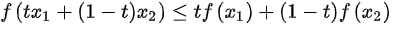
\includegraphics[scale=1]{convex}
	
	\caption[تعریف تابع محدب]{
		تعریف تابع محدب
	}
	%	\label{fig:fig-2_03}
\end{figure}
%%%%%%%%%%%%%%%%%%%%%%%%%%%%%%%%%%%%%%%%%%%
\newpage
‌